% vim:textwidth=70
\chapter{自动推断系统层次结构任务模型的方法}
\label{chap:scalpel}

\section{本章引言}

随着Internet服务逐渐渗入人们日常的生产生活,它们的可靠性也变的越来
越重要。系统设计实现上的缺陷,一直伴随着这些服务而生,导致服务性能下降,
甚至彻底中断运行。在诸多的软件缺陷(bug)中,那些最难找到和解决的是让
系统仍然运行,但是却偏离了系统期望行为的缺陷。这些缺陷的根本原因,隐藏
在复杂甚至是混乱的应用逻辑中,因此寻找并分析这些缺陷变的异常困难。

支撑Internet服务的系统本质上就非常复杂,这更增加了分析理解系统异常行为
的难度。这些系统通常使用了分层的体系结构,将其功能抽象表达为不同的层次
结构。其运行时具有高度的并发性。系统在运行时,处理着许多用户层次的
\emph{任务},例如用户请求,任务被分成许多阶段执行,不同的阶段被分布在
多个机器、进程和线程上执行,使用事件或者异步消息作为通知机制。验证单独
每个任务的行为,是一件具有挑战性的问题,因为开发人员需要重构出任务的执
行流,将任务执行过程中的各个阶段重新连接起来。

从概念上说,开发人员可以把任务执行表示为\emph{层次结构的任务模型},
这与系统的分层体系结构设计一致。不同层次的任务表示在不同阶段不同模块执
行的一段执行过程。高层任务的执行被分为若干低层子任务。\note{pacifica
example}。基于任务模型,开发人员可以更好的理解系统模块间的结构,以及不
同模块间的依赖关系,并验证处于不同层次任务的行为。

然而,目前的\note{工具}需要开发人员手动标注任务模型。例如,
Pip~\cite{pip}要求开发人员将系统预期行为,用“期望(expectations)”的
形式表达,“期望”表达了系统正确执行时的任务模型,包括对执行时资源使用
的约束。通过对比期望与实际执行的区别,可以验证系统运行时行为。写出一个
全面表达系统高层设计与底层实现的期望是非常困难的并容易出错的事情,特别
对那些正在快速发展中的系统。基于执行路径的工具,例如
Magpie~\cite{magpie},可以从单独的运行事件trace推断每个请求的执行路径,
但是它仅可以处理的一组事前确定的事件,并且需要开发人员指定任务的边界与
关联条件。

本文的目的是探索不需要人工帮助,自动推断层次结构任务模型的方法。开发人
员不需要手动标注源代码来指定任务边界,并却任务的层次结构也应该能够自动
推断得到。这样,开发人员和系统管理员就可以利用得到的任务模型,以可视化
的形式表现系统设计和实现,也可以将任务模型作为输入,使用其它工具调试或
验证系统设计。

设计一个自动任务模型的推断工具面临如下几个挑战性问题。首先,应该能够确
认合适的任务边界,这一过程应该只基于对系统执行过程的监视,而不需要开发
人员显示的标注。其次,必须能够正确的关联任务之间依赖关系。特别是,必须
能够辨别任务之间因为共享资源(例如,共享队列、锁等)而产生的依赖关系。
最后,应该能够自动恢复任务的层次结构。任务由许多或者顺序或者并行的子任
务构成。考虑到复杂系统中任务执行的非确定性,确定它们的依赖关系与层次结
构并不容易。

在本文中,我们描述了如何自动推断复杂系统层次结构任务模型的方法,并实现
了一个原型系统Scalpel。我们通过使用插装(instrument)技术来透明的观测
系统运行,获取系统运行过程的trace,包括用户和系统函数调用的过程。自动
推断方法使用trace作为输入,自下而上(bottom-up)的推断系统层次结构任务
模型,推断的过程分为三步,分别对应上面提到的三个挑战性问题。

首先,我们将运行过程分为一个个叶子任务,它们是层次结构任务模型中最基本
的任务。叶子任务的边界对应执行的同步点(synchronization point)。在同
步点,线程或进程相互同步从而具有依赖关系,因此同步点是推断任务边界的一
个合理启发点(heuristic)。

其次,我们按照运行时的因果依赖关系,将叶子任务用有向边连接,形成一个因
果关系图。叶子任务的因果依赖关系由任务运行时的执行顺序推断得到。

最后,我们在任务关系图上,推断出层次结构。每一个层次,大致对应系统设计
与实现上的一个层次。我们使用聚类算法寻找任务关系图上重复出现的模式(就
是频繁子图),以此为依据确认高层任务与构成它的子任务。通过递归的使用聚
类算法,我们能够进一步寻找更高层次的任务。

\note{prelimianry experience}

\note{文章安排}


\section{推断方法设计}

本节叙述推断方法设计,以及它的原型实现\pozhehao{}Scalpel。

\subsection{收集系统运行trace}
收集什么

全序关系?



\subsection{确定叶子任务}

在系统执行trace的基础上,我们首先需要确定叶子任务的边界。Scalpel使用
\emph{同步点}作为启发点定义任务边界。同步点是两个线程同步相互执行,从
而具有执行顺序关系的地方。在同步点,线程可能因为互斥或者相互协同而具有
顺序关系,前者的例子是线程使用锁同步对共享资源的访问,后者的例子是线程
等待另外一个线程的信号消息。

我们定义两个相继的同步点之间的执行为一个叶子任务。采用这个定义的原因是,
首先两个同步点之间的一段执行是相对独立,并且自包含的。因此,它们合理的
成为任务模型中最小粒度的一段执行,也是叶子任务的一个自然定义。另外,因
为采用了同步点定义叶子任务的边界,叶子任务之间的依赖关系也只发生在边界
之间。

Scalpel通过插装系统函数库中的同步原语(锁、信号、事件等)与socket操作
\footnote{我们认为通信也是一种同步操作。}获得相关的trace。在实际系统中
的应用经验表明,插装这些系统操作是足够的。如果应用系统使用spin-lock或
者lock-free的数据结构,则仅插装系统调用是不够的。这时Scalpel会丢失一些
同步点从而使任务模型粒度更粗。手工标注可以解决这个问题,但是整个推断方
法不再是全自动的。鉴于多数实际系统还是采用系统调用进行同步,我们将这个
问题留作将来的工作。

\subsection{任务因果关系图}

为了推断任务的层次结构,我们首先要连接叶子任务直接的依赖关系。我们使用
因果关系图。这个图中,节点表示叶子任务,有向边表示叶子任务直接的依赖关
系。\note{For example, in PacificA...}。

Scalpel使用执行顺序关系推断任务的因果依赖关系,这包括同一线程内顺序执
行的两个叶子任务,以及因为同步而依次执行的叶子任务。我们需要将“假”的
因果依赖关系区别并去除。一个“真”的依赖关系的例子是,一个从队列里取出
并处理事件的任务,在因果关系上依赖于产生那个事件并将其加入队列的任务。
另一方面,如果两个线程使用互斥锁同步对共享资源(例如I/O)的访问,虽然
它们的行为在表面上也构成因果依赖关系,但实际上,任务直接并不相互依赖,
其执行的顺序有调度器随机决定。因此,我们将互斥排除在因果关系之外。

Scalpel使用若干启发点分辨真的因果依赖关系。如果系统使用操作系统提供的
队列(例如I/O completion ports),或者通知机制(例如event),则可以使
用同步操作使用的句柄(保存在插装得到的trace中,是同步操作的参数),将
生产线程与消费线程联系起来。对于操作系统的互斥锁(mutex)与信号量
(semaphore)对象,它们通常被用来同步线程对共享资源的访问,因此不认为
它们构成因果依赖关系。

\note{即使扔了mutex问题也不大,因为只是用mutex同步访问,
producer-consumer关系可以从iocp看出来。}

\note{match socket}


\subsection{推断任务层次结构}

我们通过不断挖掘任务因果关系图上重复出现的模式,来推断任务的层次结构。
发掘算法受到文章~\cite{wpp}的启发,\cite{wpp}的工作通过搜寻“热点子路
径”(就是函数调用路径上重复出现的字串),来推断上下文无关文法。类似的,
我们的算法搜寻任务因果关系图上重复出现的子图。我们认为每一个子图都在逻
辑上代表了一个更高层的任务,它由子图中的任务集合构成。通过递归调用挖掘
算法,我们得到了层次结构的任务模型。

具体的,推断算法首先枚举任务因果关系图上所有的连通子图,并将这些子图按
照相似度(在下文中叙述)聚类为多个模式。推断算法将每个出现次数超过设定
阈值的模式定义为一个高层任务。接下来,得到的高层任务被替换为单个“超级”
节点。通过递归应用算法,我们可以得到更高层的任务,直到没有新的高层任务
产生。这时,因果关系图包括了若干超级节点,以及一些未聚类的叶子节点,图
可能是连通也可能是不连通的。Scalpel将那些超级节点输出,每个节点都是一
个最高层的任务模型。通过将超级节点展开为构成它们的子图,我们可以得到任
务的整个层次结构。

算法中使用相似度将子图聚类为不同的模式,目前,我们使用精确匹配来定义两
个子图相似,也就是两个子图完全同构。我们使用确定性的序列化算法,将子图
编码,并使用编码的哈希值将子图聚类。这个聚类算法非常有效。当编码叶子任
务时,我们使用任务两个边界上的函数调用栈作为任务的编码,忽略了任务执行
过程中调用的函数~\footnote{\note{有二义性,没弄明白,看看代码。}}。对
于同一个类中的叶子任务,它们的函数调用栈完全相同。这个方法忽略了叶子任
务的一些不重要的区别,例如函数的参数与线程号。从经验来看,这个方法很好
的区分了同一类别的叶子任务。

\note{具体算法(伪代码)}

\subsection{实现}

a

\section{讨论}

Scalpel主要是为系统开发者而设计的,希望能够帮助他们理解、验证与调试搭
建的系统。因此,我们假设程序的调试信息(主要是符号表)是可以得到的。
Scalpel利用这些信息追踪函数调用,为叶子任务提供易于理解的名字。这个假
设并不是推断任务层次结构的必要条件。即使没有调试信息,我们仍然可以对系
统调用插装,追踪同步点的调用信息。通过使用stack walking技术,我们可以
得到函数地址形式的调用栈。函数地址与函数名有对应关系,仍然可以用来分析
推断任务结构。因此,无论有没有调试信息,我们都可以推断出同样结构的层次
任务模型来。如果没有调试信息,叶子任务的名字不易于人去理解,但是不妨碍
使用其他调试工具分析任务模型。

人们习惯上使用因果路径分析~\cite{pinpoint, project5, pip, magpie}去分
析系统行为,这种方法将系统的运行过程抽象为单层的因果路径。我们认为,作
为本文核心概念的层次结构任务模型,是对因果路径分析的一个扩展。实际上,
如果只看叶子任务这一层,则我们的任务模型实际上就是因果路径,因此也可以
被用在类似的基于路径的分析中。然而,层次结构可以带来更多的好处。它将实
现细节包装在更高层次的任务中,程序员可以再不同的任务层次和粒度下,分析
验证系统行为。可以用类似Pip~\cite{pip}的方法,在不同层次的任务上,将
系统行为与程序员的期望做比较验证。虽然本文的工作侧重与推断方法的设计,
并未提出在任务模型上进一步分析的方法,我们希望能在将来的工作中完成进一
步的工作。

\section{验证推断方法}

iocp, event, mutex

\section{应用实例}

在本节,我们使用Scalpel分析一些复杂系统,以评测任务模型是否有效。可以
从两个方面来评测任务模型。首先,任务模型应该能够表达出系统设计的含义。
这一点很难用数字测量,因此,我们需要程序员去将推断的任务模型与实际系统
设计对比,判断两者是否符合。其次,任务模型也是验证系统正确性或者性能的
方法,所以,我们也可以评测任务模型在帮助调试系统时的有效性。

我们同时使用这两种方式评测Scalpel,分别将Scalpel应用在
Apache~\cite{apache}和PacificA~\cite{pacifica}上。Apache和PacificA都使
用了典型的配置。我们在Apache上增加了一个Subversion(SVN)模块,并使用
客户端执行10次checkout。我们使用两台机器配置了一个PacificA的复制组
(Replication Group),一台机器时主节点(primary),一台是从节点
(backup)。我们运行一个测试程序,在Pacifica中创建一个表,并提交15条随
机数据。我们使用Scalpel追踪每个系统的运行,并推断任务模型。两个实验都
是在如下机器配置上进行的:2.0 GHz Xeon双核CPU,4 GB内存,运行Windows
Server 2003 SP2操作系统,机器间通过1 Gb网络连接。

\subsection{Apache}

我们首先人工验证Scalpel在Apache上推断的任务模型。图~
\ref{fig:apache_model}显示了得到的模型。在图上,每个节点都是一个叶子任
务,连接任务的实线与虚线表示任务之间的因果关系,实线表示线程内部执行顺
序因果关系,虚线表示线程间因果关系。叶子任务上标记了任务起始点的调用栈。
为了易于理解,在本文中,我们只显示了调用栈尾部调用同步函数的那个函数名
称。

\begin{figure}
\centering
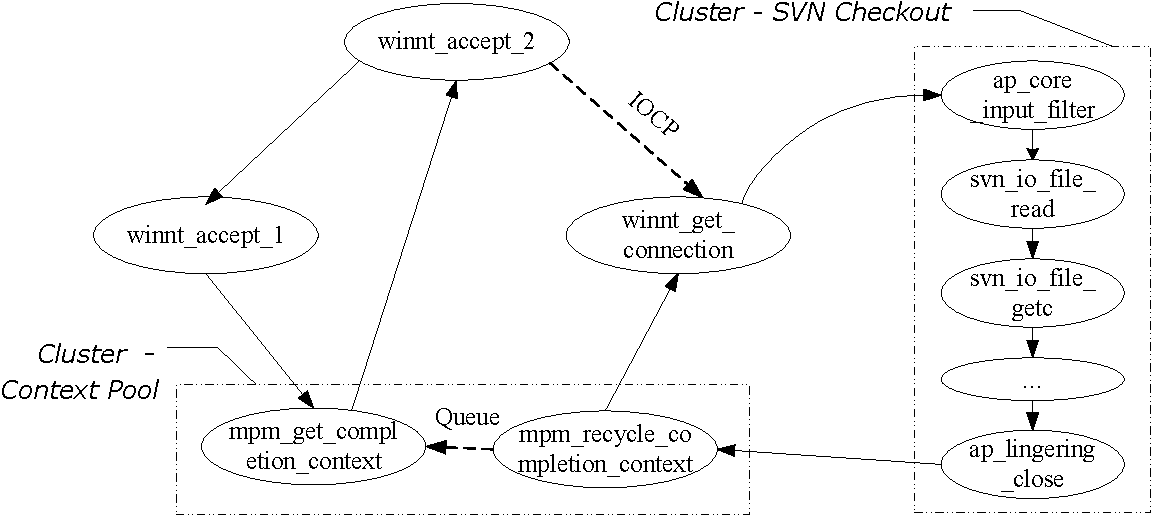
\includegraphics[width=\linewidth]{apache-task-model}
\caption{执行SVN checkout得到的Apache任务模型}
\label{fig:apache_model}
\end{figure}


通过仔细阅读理解Apache和SVN的代码,我们确定推断的模型就是Apache服务SVN
checkout操作时的工作流程。Apache接受外来的请求,并将请求交给线程池中的
一个worker线程去完成。Scalpel推断出5个Apache核心执行的叶子任务(图~
\ref{fig:apache_model}的左边部分)。每个任务表示Apache接受并服务请求的
主要步骤。详细说,监听线程接受连接(\texttt{winnt\_accept\_1}),从连
接上下文\footnote{Connection context,描述外来请求的数据结构。}资源池
中取出一个连接上下文(\texttt{mpm\_get\_completion\_context}),并将这
个上下文通过I/O completion port(IOCP)传递给worker线程
(\texttt{winnt\_accept\_2}),并继续等待其他请求到来。在IOCP的另一边,
线程池中的一个worker线程首先获得连接上下文
(\texttt{winnt\_get\_connection}),并调用SVN服务模块去处理请求(从
\texttt{ap\_core\_input\_filter}到\texttt{ap\_lingering\_close})。之
后,worker线程将连接上下文回收到上下文资源池
(\texttt{mpm\_recycle\_completion\_context}),并等待IOCP中的其它请求。
SVN checkout过程中的一些叶子任务未在图上完全显示,但是它们都是处理请求
过程中的关键步骤。因此,这也是使用同步点为启发推断叶子任务边界有效性的
一个例证。

进一步的,Scalpel还成功的找到了两个有实际含义的高层任务,见图~
\ref{fig:apache_model}中方框表示的部分,在图上我们按照两个任务的工作给
它们标了名字。第一个高层任务(Context Pool)包括了连接上下文被取出用来
传递用户请求又被回收的过程。另一个(SVN checkout)包含了SVN checkout被
处理的过程。因为这两个任务都被频繁执行,因此Scalpel可以精确的将他们确
认为高层任务。

\subsection{PacificA}

图xxx

% 把secondary也加上

图xxx显示了PacificA的任务模型。PacificA开发者确认了这个模型准确表达了
用户提交数据在主节点上执行的过程。模型包含了三个高层任务,分别是提交数
据执行过程的三个主要步骤:一个worker任务,一个本地提交任务和一个确认远
程提交的任务。在worker任务中,一个socket监听线程循环的等待用户请求
(\texttt{Session\-::Recv\-Packet}),接受来自用户的消息,并将用户请求
通过IOCP交给线程池中的worker线程去执行
(\texttt{PA\-Thread\-Pool\-::Thread\-Internal\-::DoWork})。worker线
程取到用户请求后,立即执行本地提交任务。它首先将数据在本地存储
(\texttt{Logic\-Replica\-::Mutate},并将提交请求使用异步RPC发送给从节
点(\texttt{Rpc\-Client\-::Rpc\-Async\-Call\-Chain}),RPC被序列化后通
过网络层发送出去(\texttt{Session\-::Send\-Packet}),在主节点确认自己
已经持久化存储用户提交数据后
(\texttt{Logic\-Replica\-::Receive\-MutationAck}),本地提交任务结束。
从节点在收到提交请求后将数据存储,并给主节点发确认命令
(acknowledgement)。确认远程提交任务就是主节点处理从节点确认命令的。
它首先处理从节点的确认消息
(\texttt{Logic\-Replica\-::Receive\-Mutation\-Ack}),之后向用户回复
数据提交请求的结果(\texttt{Rpc\-Client\-::Rpc\-Call\-Reply}),RPC被
序列化后通过网络层发送出去(\texttt{Session\-::Send\-Packet})。

值得注意的是,Scalpel不仅仅能够推断出用户提交数据的过程可以分为三个高
层任务,同时能够将worker线程执行的本地提交和确认远程提交两个任务区分开
来。这不是因为Scalpel理解了任务执行的语意,而是因为,这两个任务分别被
两次\texttt{DoWork}任务触发执行,因此,挖掘算法能够将每个任务正确的区
分开来。

\begin{table}[t!]
\small
\centering
\caption{Statistic numbers of Apache and PacificA.}
\label{scp:statistics}
\begin{tabular}{lll}

  		& Apache	& PacificA \\
\hline
Leaf Tasks	& 423952	& 10636 \\
\hline
Events		& 0			& 47 \\
Mutex 		& 210472	& 4950 \\
IOCP		& 23		& 16 \\
Socket		& 527		& 77 \\
run-after	& 193972	& 11304 \\
\hline

\end{tabular}
\end{table}

表~\ref{scp:statistics}小结了推断算法的执行统计。

接下来,我们评测使用Scalpel得到的任务模型对帮助调试系统是否有效。
PacificA的开发者希望我们能够使用Scalpel帮助他们解决系统中的一个性能问
题。开发者注意到了这个问题,并曾经试图使用函数性能概要分析(profiling)
的办法,但是没有解决问题。我们使用图~\ref{pacifica-model}的模型分析
PacificA的性能。对每一个叶子任务,我们使用Scalpel记录它的执行时间,网
络带宽消耗,CPU使用等信息。对高层任务,我们将它的子任务性能参数聚集得
到它的性能参数信息。

通过在压力测试中执行数据提交操作,我们很快发现了那个性能问题:提交任务
很难使用所有的网络带宽,同时它的CPU使用率也很低,远小于100\%。我们通过
自上而下的办法找到这个问题的症结,从最高层任务向下,找到执行时间最长的
那个任务。我们发现,当以很高频率发送数据时,发送线程(典型的配置是4个
并行线程同时发送)会在某一时刻阻塞大约一秒钟,其原因是,在PacificA的网
络层代码,会对数据发送做流量控制,如果发送消息的缓冲区慢了的话,流量控
制会引起所有发送线程同步sleep一秒,如图~\ref{flow_control_code}。这样,
四个并发的发送线程就会表现出几乎同步的行为来,如图~\ref{sleep_send}所
示。

进一步对代码审查让我们对问题根本原因有了深刻理解。当使用异步方式调用
RPC时,RPC层并没有流量控制机制。每个发送线程都会以非阻塞方式独立发送
RPC消息。网络层的消息缓冲区很快就会被填满,导致发送线程被网络层阻塞(
图~\ref{flow_control_code})。这就让发送线程表现出了同步的行为,无论使
用多少RPC发送线程,它们都会被在网路层被同步阻塞。引起这个问题的根本原
因是RPC层和网络层没有一致的控制逻辑。通过使用层次结构任务模型,我们很
快能够找到性能问题,并理解造成它的根本原因。

% statistics

\section{性能评测}

overhead, script run time, 


\section{相关工作}

a

\section{本章小结}

a

